%#######################################################################
% German task description for task "cache"
%
% Copyright (C): 2018, HAUER Daniel, daniel.hauer@tuwien.ac.at
% License GPL V2 or later (see http://www.gnu.org/licenses/gpl2.txt)
%#######################################################################

\documentclass[a4paper,12pt]{article}
\usepackage{a4wide}
\usepackage{tikz}
\usetikzlibrary{calc}
\usepackage[ngerman]{babel}

\begin{document}
\pagestyle{empty}
\setlength{\parindent}{0em} 
\section*{\noindent Cache }

Ihre Aufgabe ist es, das Verhalten einer Entity  namens "`cache"' zu programmieren. Die Entity ist in der angeh\"angten Datei "`cache.vhdl"' deklariert und hat folgende Eigenschaften:

\begin{itemize}
	\item Eingang: addr vom Typ std\_logic\_vector mit L\"ange {{addr_length}}
	\item Eingang: en\_read vom Typ std\_logic
	\item Eingang: clk vom Typ std\_logic
	\item Ausgang: data vom Typ std\_logic\_vector mit L\"ange {{data_length}}
	\item Ausgang: ch\_cm vom Typ std\_logic

\end{itemize}

\begin{center}
\begin{tikzpicture}
\draw node [draw,rectangle, minimum height=24mm, minimum width=35mm,rounded corners=2mm,thick](entity){};

\draw[->] ($ (entity.west)+(-10mm,6.0mm)$) -- ($ (entity.west) + (0mm,6.0mm)$);
\draw[anchor=east] node at ($ (entity.west)+(-9mm,6.0mm)$){ addr };

\draw[->] ($ (entity.west)+(-10mm,0.0mm)$) -- ($ (entity.west) + (0mm,0.0mm)$);
\draw[anchor=east] node at ($ (entity.west)+(-9mm,0.0mm)$){ en\_read };

\draw[->] ($ (entity.west)+(-10mm,-6.0mm)$) -- ($ (entity.west) + (0mm,-6.0mm)$);
\draw[anchor=east] node at ($ (entity.west)+(-9mm,-6.0mm)$){ clk };


\draw[->] ($ (entity.east) + (0mm,4.0mm)$) -- ($ (entity.east) + (10mm,4.0mm)$);
\draw[anchor=west] node at ($ (entity.east) + (9mm,4.0mm)$){ data };

\draw[->] ($ (entity.east) + (0mm,-4.0mm)$) -- ($ (entity.east) + (10mm,-4.0mm)$);
\draw[anchor=west] node at ($ (entity.east) + (9mm,-4.0mm)$){ ch\_cm };


\draw node at ($ (entity) - (0,0mm)$){ cache };

\end{tikzpicture}
\end{center}

Ver\"andern Sie die Datei "`cache.vhdl"' nicht!\\




Ziel dieser Aufgabe ist es, die Leseeinheit eines \textit{direct mapped} Caches zu programmieren. Abh\"angig von der angelegten Adresse am Adresseingang \textit{addr} des Caches soll dieser durchsucht und bei einem \textit{cache hit} der Speicherinhalt ausgegeben werden. Bei einem \textit{direct mapped} Cache ist die Position eines Datums im Cache eindeutig \"uber die Adresse definiert. Umfasst der Cache M Eintr\"age, so werden N = log2(M) Bits der Adresse f\"ur die Positionbestimmung (Index) im Cache ben\"otigt und die restlichen Bits der Adresse als \textit{Tag} zu dem Datum im Cache dazugespeichert. Bei der \"Uberpr\"ufung, ob ein Datum im Cache vorhanden ist, muss also zun\"achst die Position im Cache anhand eines Teilst\"ucks der Adresse ermittelt und anschlie{\ss}end der gespeicherte Tag mit dem zweiten Adressteil verglichen werden. Nur wenn dieser \"ubereinstimmt, liegt ein \textit{cache hit} vor. Abbildung \ref{img_cache} verdeutlicht das Prinzip eines \textit{direct mapped} Caches. \\

\begin{figure}[h]
\begin{center}
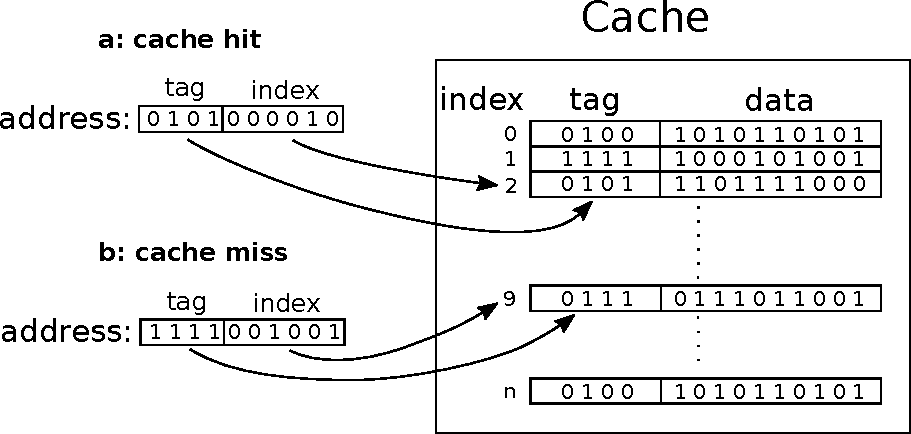
\includegraphics[width=0.75\textwidth]{../static/cache.pdf}
\caption{Prinzip des Lesezugriffs bei einem \textit{direct mapped} Caches. (Dies ist eine exemplarische Darstellung, die Bitbreiten stehen in keinem Zusammenhang zu Ihrer Angabe.)}
\label{img_cache}
\end{center}
\end{figure}

Die Cache Entity soll dabei folgende Aufgaben erf\"ullen:

\begin{itemize}

\item Der Cache soll bei

fallender

steigender

 Flanke des Takteinganges \textit{clk} arbeiten. D.h. die Ausg\"ange d\"urfen sich nur bei einer

fallenden

steigenden

 Flanke ver\"andern.

\item Ein Zugriff auf den Cache erfolgt nur, wenn \textit{en\_read} gleich '1' ist, anderenfalls soll der Ausgang \textit{data} immer hochomig (High Impedance = 'Z') sein und das Flag \textit{ch\_cm} immer '0' liefern.

\item Die im Cache gespeicherten {{cache_size}} Daten und deren Tags sind in Tabelle \ref{tab_cachedata} vorgegeben und sollen von Ihnen konstant eingespeichert werden. (Diese w\"urden von einer Schreibe-Einheit entsprechend beschrieben werden).

\item Erfolgt ein Lesezugriff (\textit{en\_read} = '1'), so soll aus der Adresse \textit{addr} die m\"ogliche  Position des Datum im Cache (Cache-Index) und der zugeh\"orige Tag ermittelt werden. Kommt es dabei zu einem \textit{cache hit}, so soll das Datum dieser Adresse am Ausgang \textit{data} ausgegeben werden und das Flag \textit{ch\_cm} auf '1' gesetzt werden. Kommt es zu einem \textit{chache miss}, so soll der Ausgang \textit{data}  hochomig (High Impedance = 'Z') sein und das Flag \textit{ch\_cm} '0' liefern. 

\item Ist bei einem Lesezugriff der Cache-Index der Adresse gr\"o{\ss}er als die Speichertiefe des Caches, so soll ebenfalls der Ausgang \textit{data}  hochomig (High Impedance = 'Z') sein und das Flag \textit{ch\_cm} '0' liefern. 

\item F\"ur die Berechnung des Cache-Index und des Tags aus der angelegten Adresse gilt au{\ss}erdem: Der Index berechnet sich aus den n niederwertigsten Adressbits, wobei n die minimal n\"otige Anzahl an Bits zur Darstellung aller {{cache_size}} Indizes im Cache ist. Die restlichen m Bits werden als Tag gespeichert (n + m = Adressl\"ange = {{addr_length}}). 

\end{itemize}

\begin{table}
\centering
\begin{tabular}{|c|c|c|}
\hline
~Cache Index~ & ~~~Tag~~~ & ~~~Data~~~ \\
\hline

{{i}}   & {{tag_values[i]}} & {{data_values[i]}} \\

\hline
\end{tabular}

\caption{Inhalt des Caches. Die Daten und Tags sind jeweils mit MSB first angegeben.}
\label{tab_cachedata}
\end{table}

Dieses Verhalten muss in der angeh\"angten Datei "`cache\_beh.vhdl"' programmiert werden.


Um Ihre L\"osung abzugeben, senden Sie ein E-Mail mit dem Betreff "`Result Task {{TASKNR}}"' an {{SUBMISSIONEMAIL}} und h\"angen Ihre Datei ``cache\_beh.vhdl'' an.

\vspace{0.7cm}
Viel Erfolg und m\"oge die Macht mit Ihnen sein.

\end{document}
